\section{Evaluation}
\label{sec:eval}
In this section, we evaluate the performance of our scheduler under a variety of workloads.

\subsection{Experimental Setup}

\textbf{Model and server configurations.} We use Qwen \cite{qwen} models with 2B, 8B, and 13B parameters, LLama3 \cite{llama3modelcard} with 7B and 8B parameters, and LongChat \cite{longchat2023} with 13B parameters. For all of our experiments, we use the RTX6000 Ada Generation GPU \cite{nvidia_rtx6000_datasheet} with an HBM of 48GB and an L2 cache size of 96MB.

\textbf{Workloads:} Similar to prior work, the arrival pattern of requests is generated by a Poisson process. The input lengths and output lengths of requests are sampled from the following real-world datasets.

L-Eval \cite{an2023leval}: It contains human-labeled query-response pairs on diverse tasks, such as summarization and question answering. The range of sequence length in this dataset is 2.7K - 210.5K tokens.

LongBench \cite{bai2024longbench2} encompasses a curated subsample of elongated data, ranging from 4K to 10K context length, excerpts from 21 datasets across 6 categories, including tasks like multi-document question answering, summarization, and code completion.


\textbf{Baseline 1: vLLM \cite{kwon2023efficient}} vLLM is a high-throughput LLM serving system designed to improve GPU memory efficiency during autoregressive decoding. Its core contribution is PagedAttention, an attention mechanism that stores the key–value (KV) cache in fixed-size blocks rather than contiguous memory. Inspired by virtual memory paging in operating systems, PagedAttention allows KV blocks to be allocated on demand and mapped non-contiguously in GPU memory, substantially reducing internal and external fragmentation caused by variable-length prompts and outputs. In addition, vLLM supports KV cache sharing across sequences. We use vLLM version 0.14.0 across all our experiments.

\textbf{Baseline 2: SGLANG \cite{zheng2024sglangefficientexecutionstructured}}
\textcolor{red}{too long, but description necessary as we can't cite anything, SGLANG's paper does not mention about the newer scheduler policies, and we need to show it as a bad design for our chunked hash tree idea to come out}
 SGLANG is a system for efficient execution of structured language model programs, consisting of a Python-embedded frontend language and a co-designed runtime. On the runtime side, SGLANG introduces RadixAttention, which enables automatic KV cache reuse across multiple generation calls by organizing cached prefixes in a radix tree with cache-aware scheduling. This allows SGLANG to exploit multi-level prefix sharing beyond simple system-prompt reuse. We use SGLANG version 0.5.7 across all our experiments.

SGLANG supports multiple request scheduling policies that trade off fairness, throughput, and KV-cache efficiency. These policies fall into two categories: cache-aware and cache-agnostic.
\begin{itemize}
    \item \textbf{Cache-aware policies.} These policies explicitly leverage the radix-tree prefix cache to increase KV reuse:
    \begin{itemize}
        \item \textbf{Longest Prefix Match (LPM):} Prioritizes requests whose input prefixes match the longest cached prefixes. This maximizes immediate KV cache reuse and reduces redundant prefill computation.
        \item \textbf{DFS-Weight:} Traverses the radix cache tree in a depth-first manner and prioritizes branches with more active requests. This groups requests that share deeper prefixes, improving cache locality over time.
    \end{itemize}
    \item \textbf{Cache-agnostic policies.} These policies do not consider prefix sharing and serve as simpler baselines:
    \begin{itemize}
        \item \textbf{First-Come-First-Serve (FCFS):} Schedules requests in arrival order. This is also the fallback policy when prefix caching is disabled.
        \item \textbf{Longest Output First (LOF):} Prioritizes requests with larger maximum generation lengths, which can improve GPU utilization under heavy load.
        \item \textbf{Random:} Randomly shuffles pending requests and is mainly used as a control or stress-test policy.
    \end{itemize}
    \item \textbf{Additional scheduling mechanisms.} In addition to request ordering, SGLANG includes:
    \begin{itemize}
        \item \textbf{In-batch prefix caching:} Detects shared prefixes among waiting requests and temporarily deprioritizes redundant ones so that a single request can populate the cache for others.
        \item \textbf{Priority-aware scheduling:} Allows requests to be assigned priorities, which can be combined with FCFS or LOF ordering.
        \item \textbf{Priority-based preemption:} Enables higher-priority requests to preempt running lower-priority ones when token or memory budgets are limited.
    \end{itemize}
\end{itemize}

\textbf{Baseline 3: Dynamic Batching \cite{pang2025optimizing}.} 
\textcolor{red}{not necessary as a baseline, not relevant?} Dynamic batching treats the batch size as a runtime decision variable rather than a fixed hyper-parameter. It continuously adjusts the active batch size based on real-time GPU memory utilization and, optionally, decoding latency constraints. The approach employs a memory-aware batch scheduler to prevent KV-cache overcommitment and a latency feedback mechanism to satisfy service-level agreements (SLAs). We implement dynamic batching onin top of vLLM as another scheduler.


\textcolor{red}{
can add more baselines?
\begin{itemize}
    \item fasttree: code not available, for end-to-end inference
    \item batchllm: does not operate in dynamic workload settings, can compare it with in a batch like setting? again code not available
    \item promptcache: maintains a database of kv cache, not directly related to our stuff?
    \item sarathi serve: can add as a baseline, which is below vllm fcfs, but not relevant otherwise?
    \item pod attention: some kind of parallel optimization, although to use, we will have to implement stuff on sarathi serve
    \item loong serve and other baselines: go through dropbox and recent conference releases again to find more stuff (TODO)
\end{itemize}
}



\textbf{Key Metrics.} Throughput (req/s) measures how many requests the system can complete per second and indicates its overall serving capacity. Higher throughput indicates better utilization of GPU compute and memory resources.

Time Between Tokens (TBT) is the average time gap between consecutive generated tokens during decoding. It reflects how smoothly and responsively the model produces output, which is especially important for interactive settings.

End-to-end latency measures the total time from when a request is submitted until the full response is generated, including both prefill and decoding stages. This metric directly captures the user-perceived response time.

Normalized latency is defined as the end-to-end latency divided by the output sequence length. It helps account for varying response lengths and enables a fair comparison across different workloads.

\textcolor{red}{out tokens/sec needed?}

\begin{figure}[H]
    \centering
    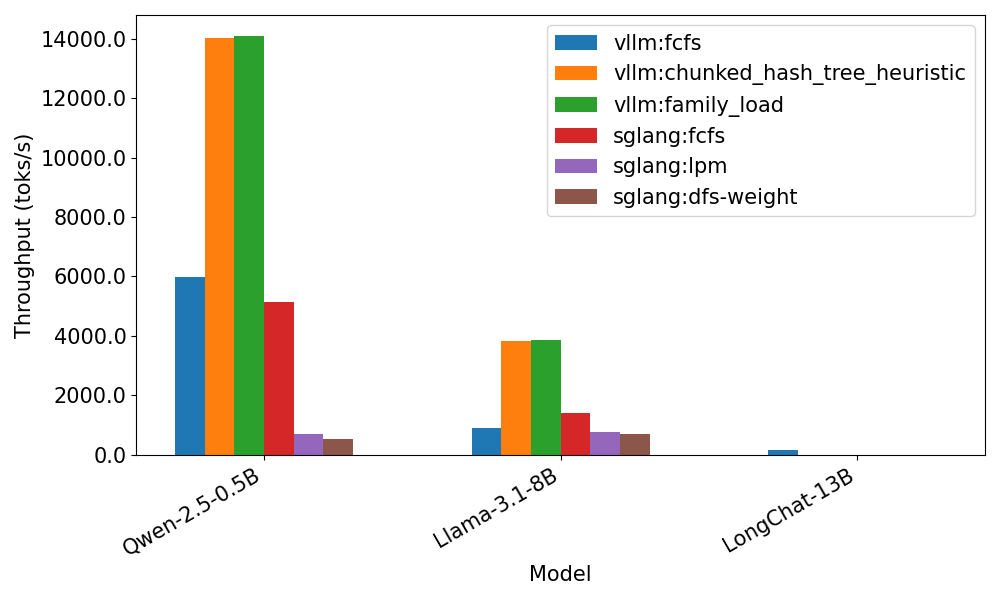
\includegraphics[width=0.8\linewidth]{results/throughput_vs_models_length_5000_families_5.png}
    \caption{Throughput comparison for various models under different scheduling policies with average shared context length of 5000 tokens and 5 prefix groups}
    \label{fig:throughput-models-len5000-fam-5}
\end{figure}

\begin{figure*}[t]
\centering
\begin{subfigure}{0.32\textwidth}
    \centering
    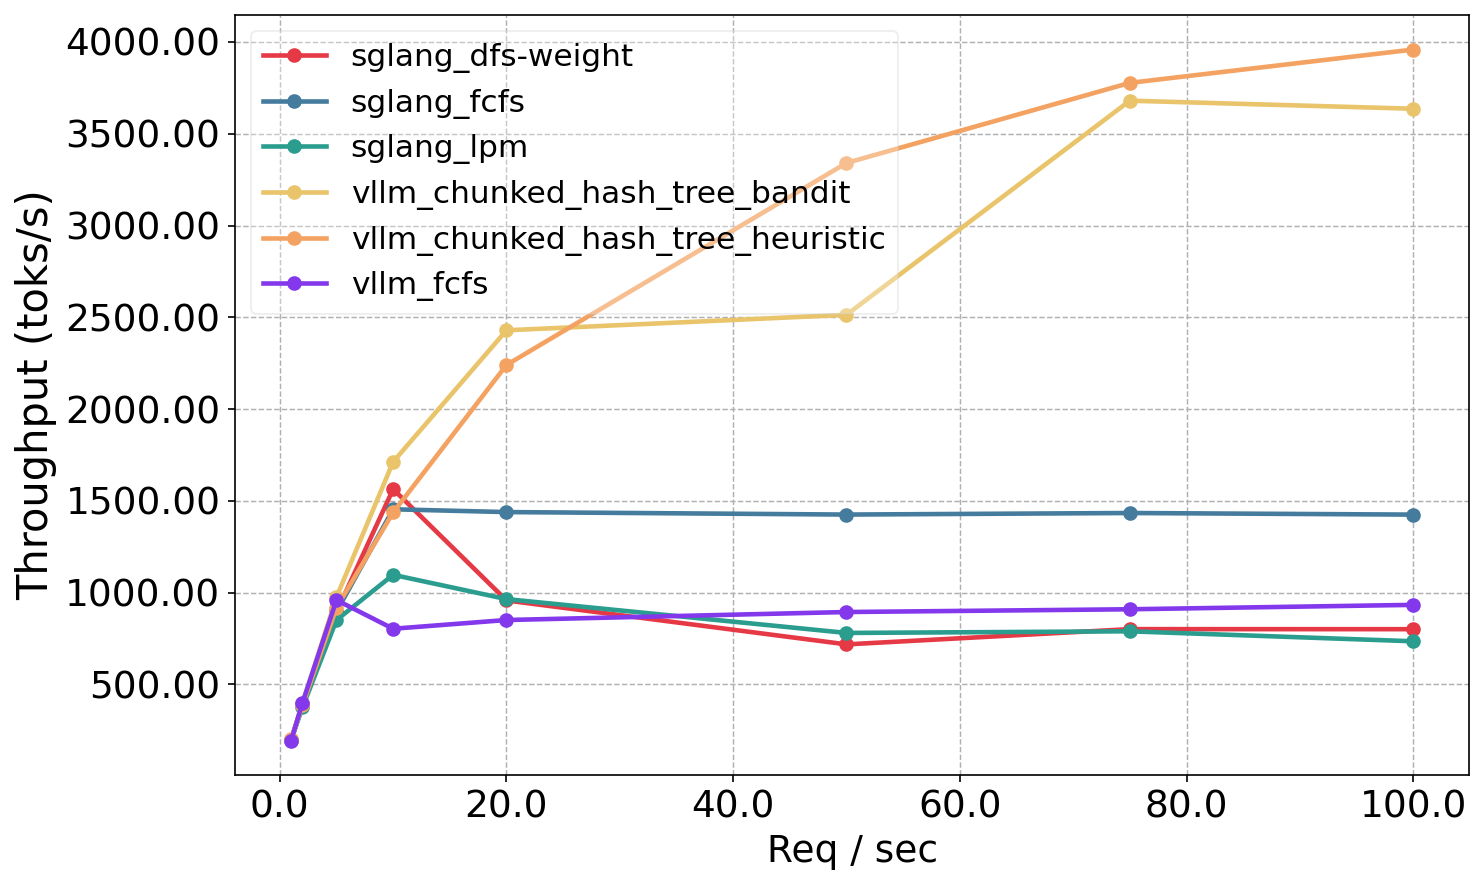
\includegraphics[width=\linewidth]{results/req_per_sec_plots/throughput_vs_rps.png}
    \caption{}
    \label{fig:tp_vs_rps_l_5000_fam_5}
\end{subfigure}
\hfill
\begin{subfigure}{0.32\textwidth}
    \centering
    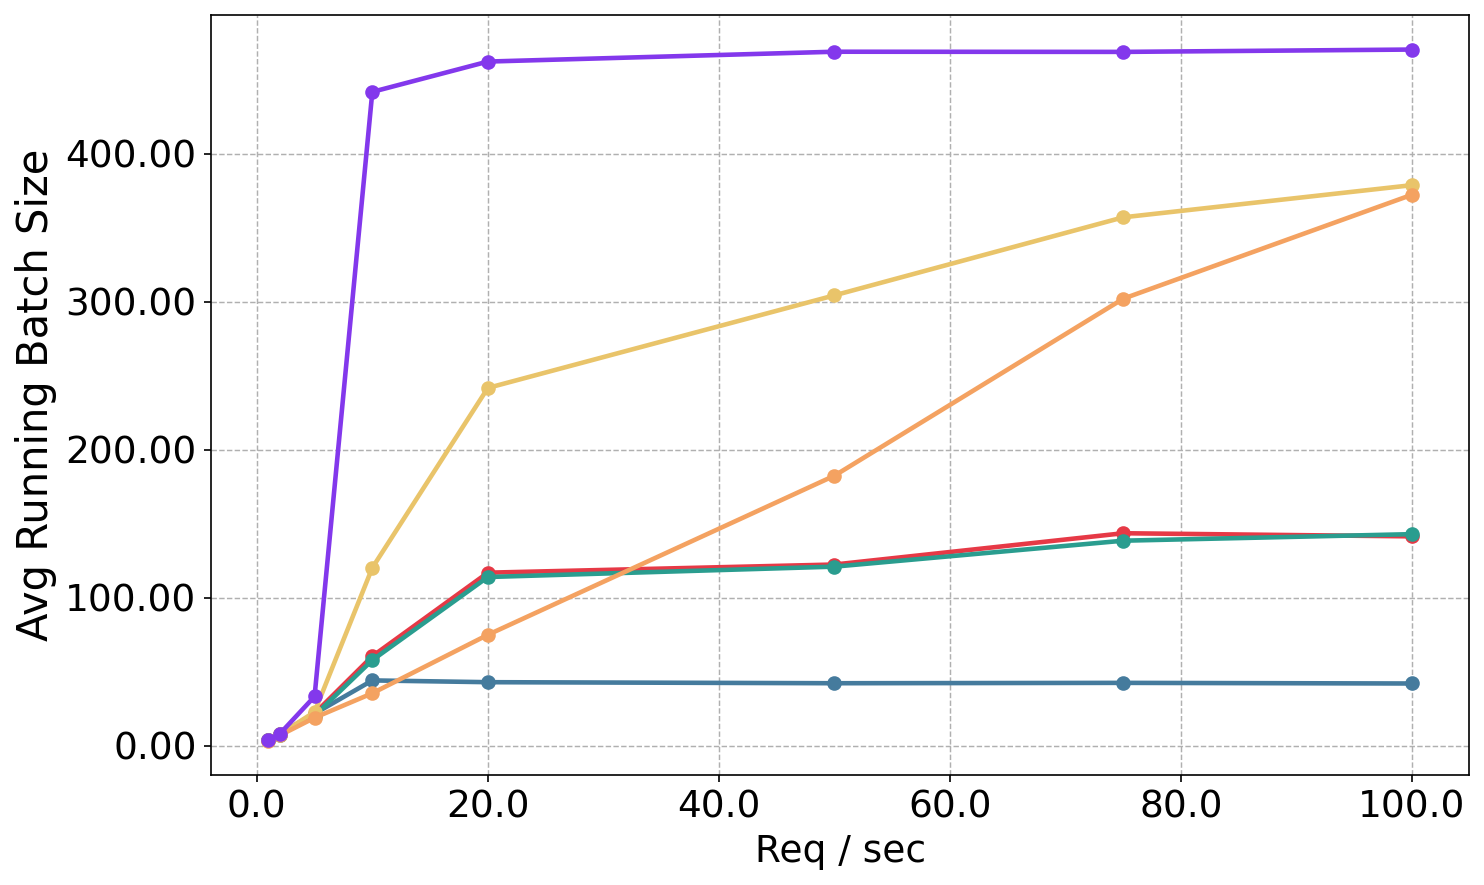
\includegraphics[width=\linewidth]{results/req_per_sec_plots/avg_batch_vs_rps.png}
    \caption{}
    \label{fig:tbt_vs_rps_l_5000_fam_5}
\end{subfigure}
\hfill
\begin{subfigure}{0.32\textwidth}
    \centering
    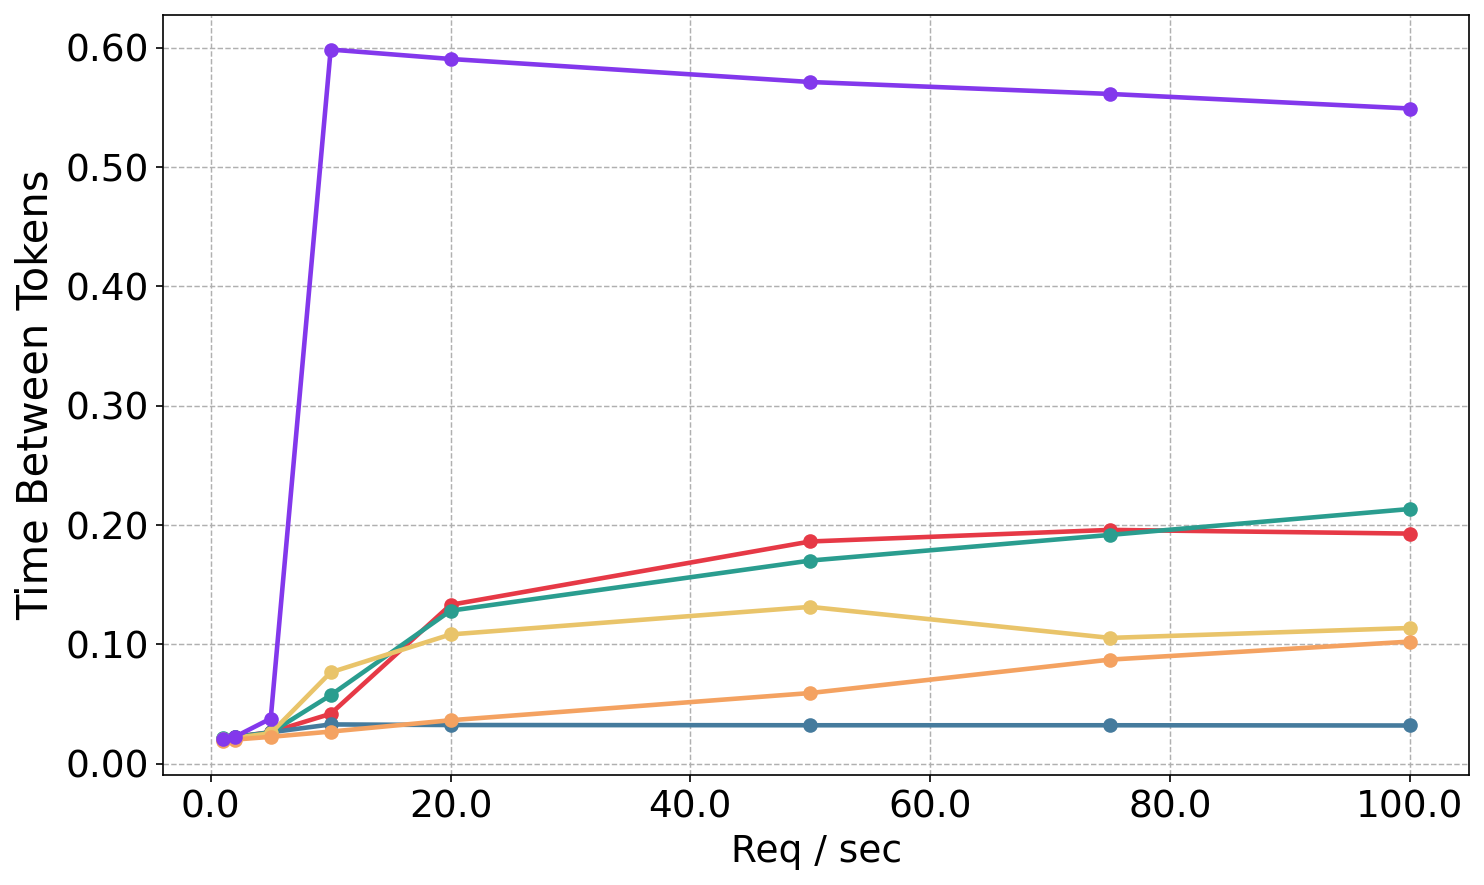
\includegraphics[width=\linewidth]{results/req_per_sec_plots/avg_timediff_vs_rps.png}
    \caption{}
    \label{fig:abs_vs_rps_l_5000_fam_5}
\end{subfigure}

\caption{Various metrics across varying input workload poisson rates. Shared prefix length of 5000 tokens; 5 prefix groups and 200 tokens decode length.}
\label{fig:metrics_vs_rps_l_5000_fam_5}
\end{figure*}

\begin{figure*}[t]
\centering
\begin{subfigure}{0.32\textwidth}
    \centering
    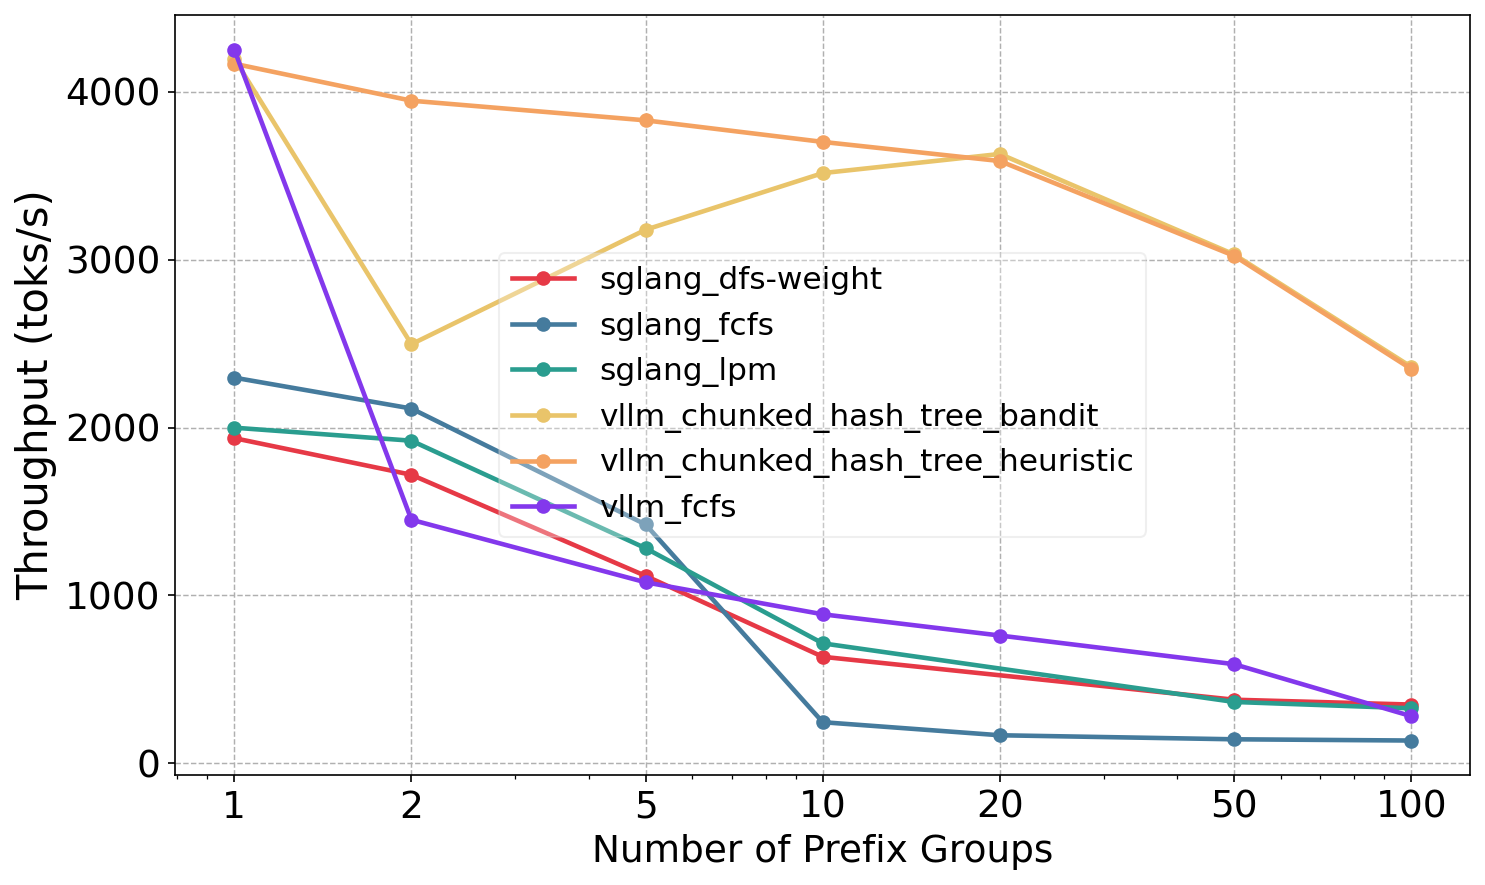
\includegraphics[width=\linewidth]{results/families_plots/throughput_vs_fam.png}
    \caption{}
    \label{fig:tp_vs_fam_l_5000}
\end{subfigure}
\hfill
\begin{subfigure}{0.32\textwidth}
    \centering
    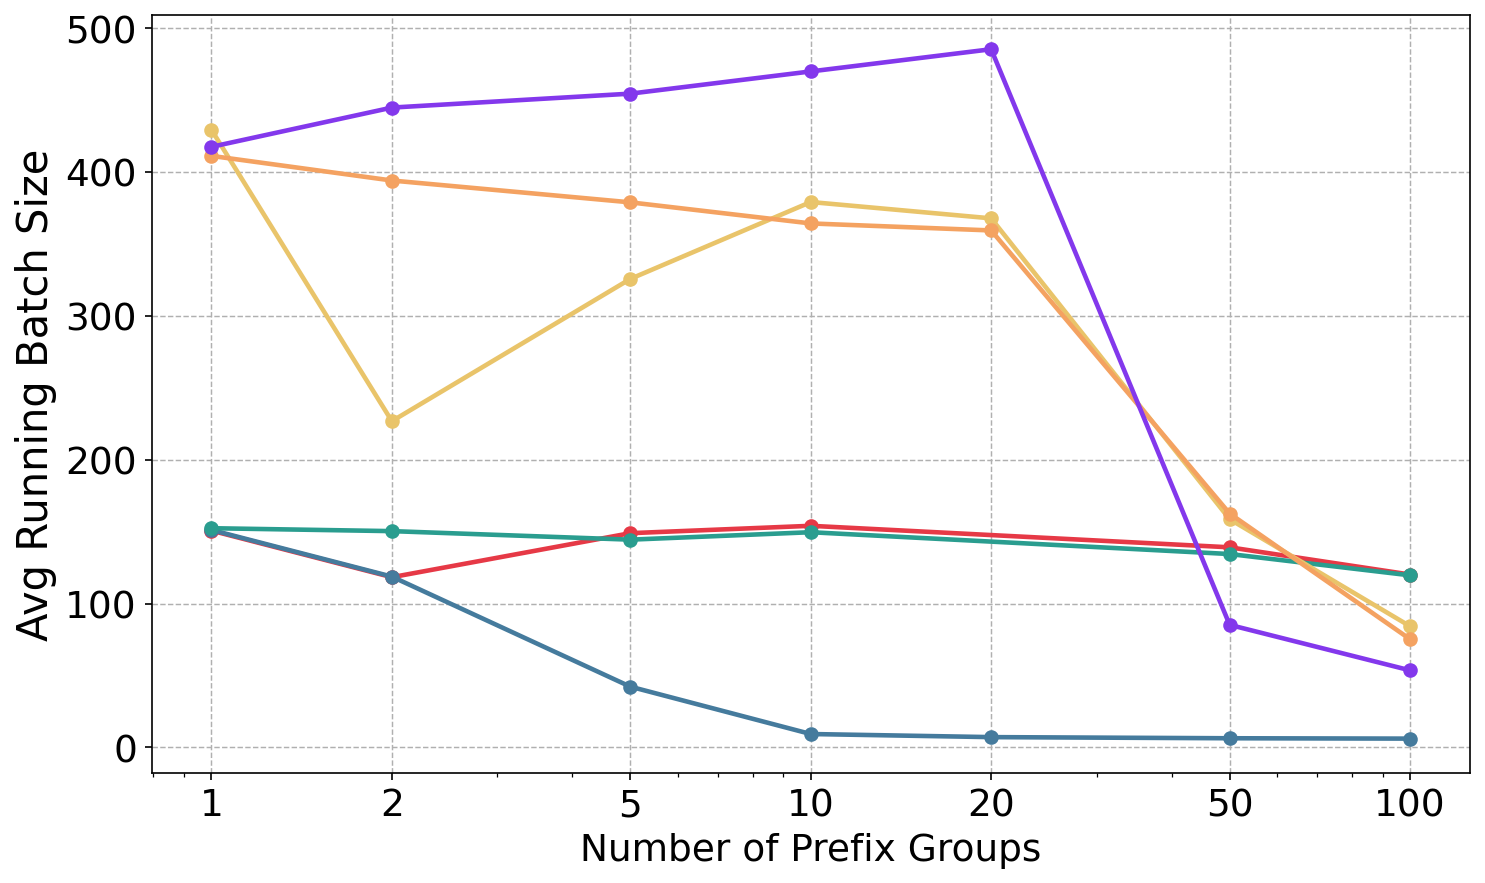
\includegraphics[width=\linewidth]{results/families_plots/avg_batch_vs_fam.png}
    \caption{}
    \label{fig:tbt_vs_fam_l_5000}
\end{subfigure}
\hfill
\begin{subfigure}{0.32\textwidth}
    \centering
    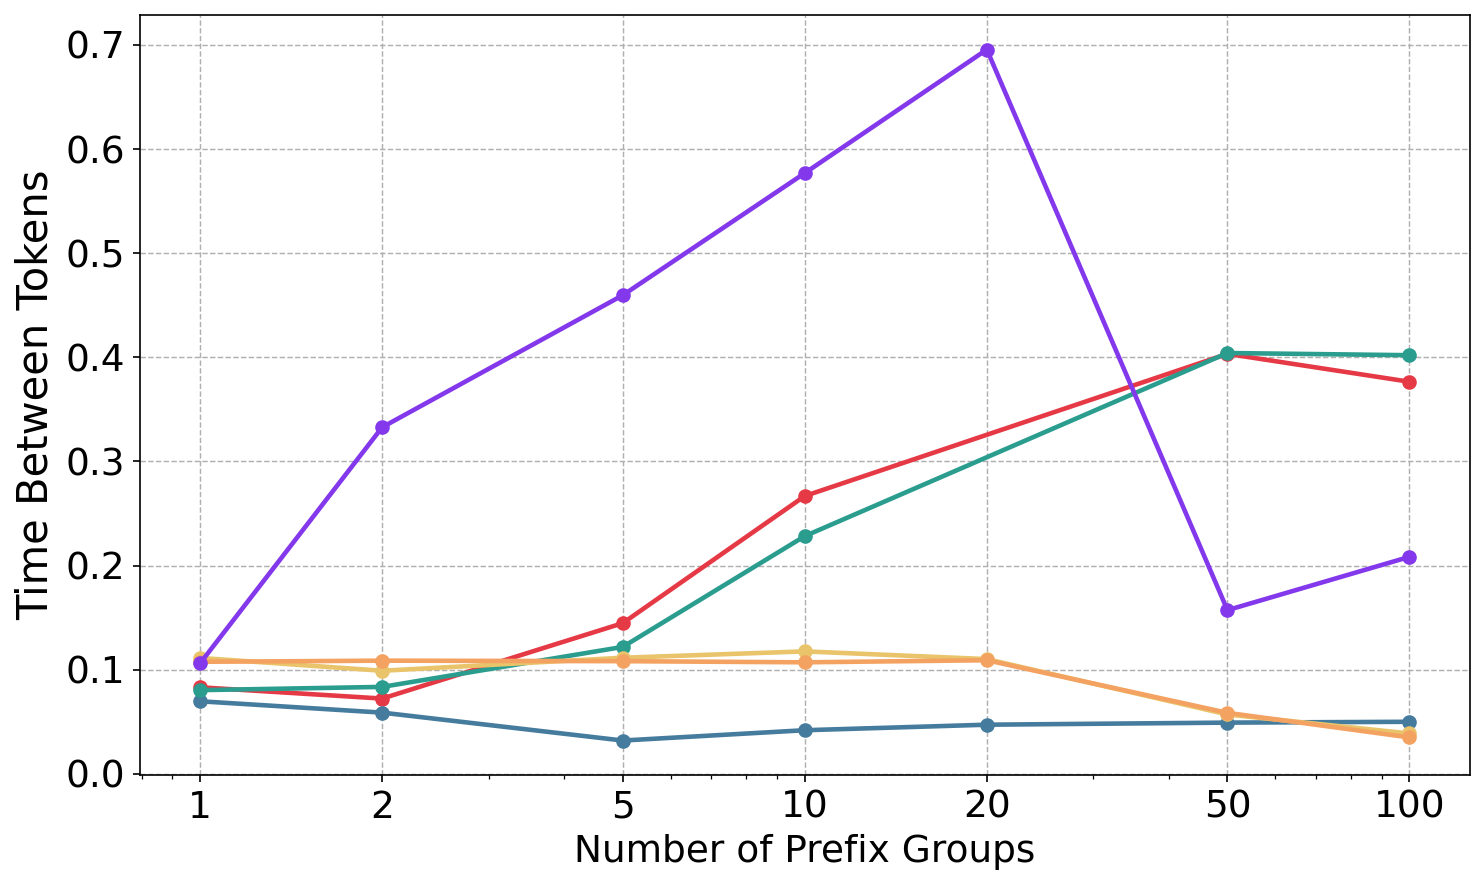
\includegraphics[width=\linewidth]{results/families_plots/avg_timediff_vs_fam.png}
    \caption{}
    \label{fig:abs_vs_fam_l_5000}
\end{subfigure}

\caption{Various metrics across varying number of prefix groups. Shared prefix length of 5000 tokens; 500 input request poisson rate and 200 tokens decode length.}
\label{fig:metrics_vs_fam_l_5000}
\end{figure*}

\begin{figure*}[t]
\centering
\begin{subfigure}{0.32\textwidth}
    \centering
    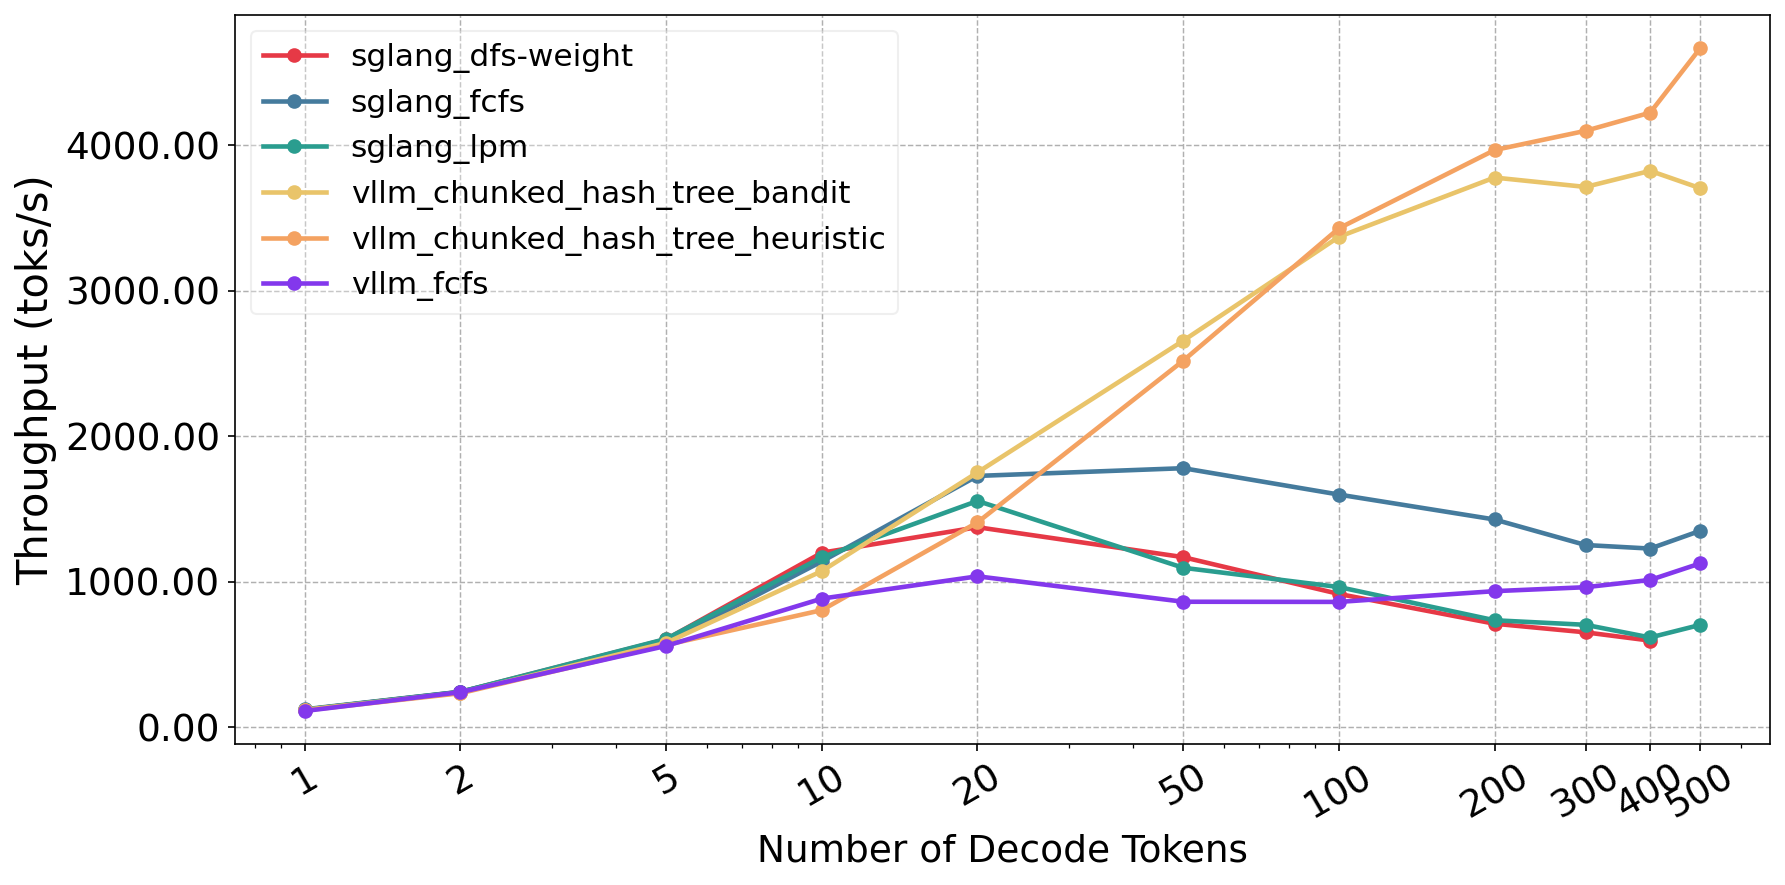
\includegraphics[width=\linewidth]{results/decode_tokens_plots/throughput_vs_tok.png}
    \caption{}
    \label{fig:tp_vs_tok_l_5000}
\end{subfigure}
\hfill
\begin{subfigure}{0.32\textwidth}
    \centering
    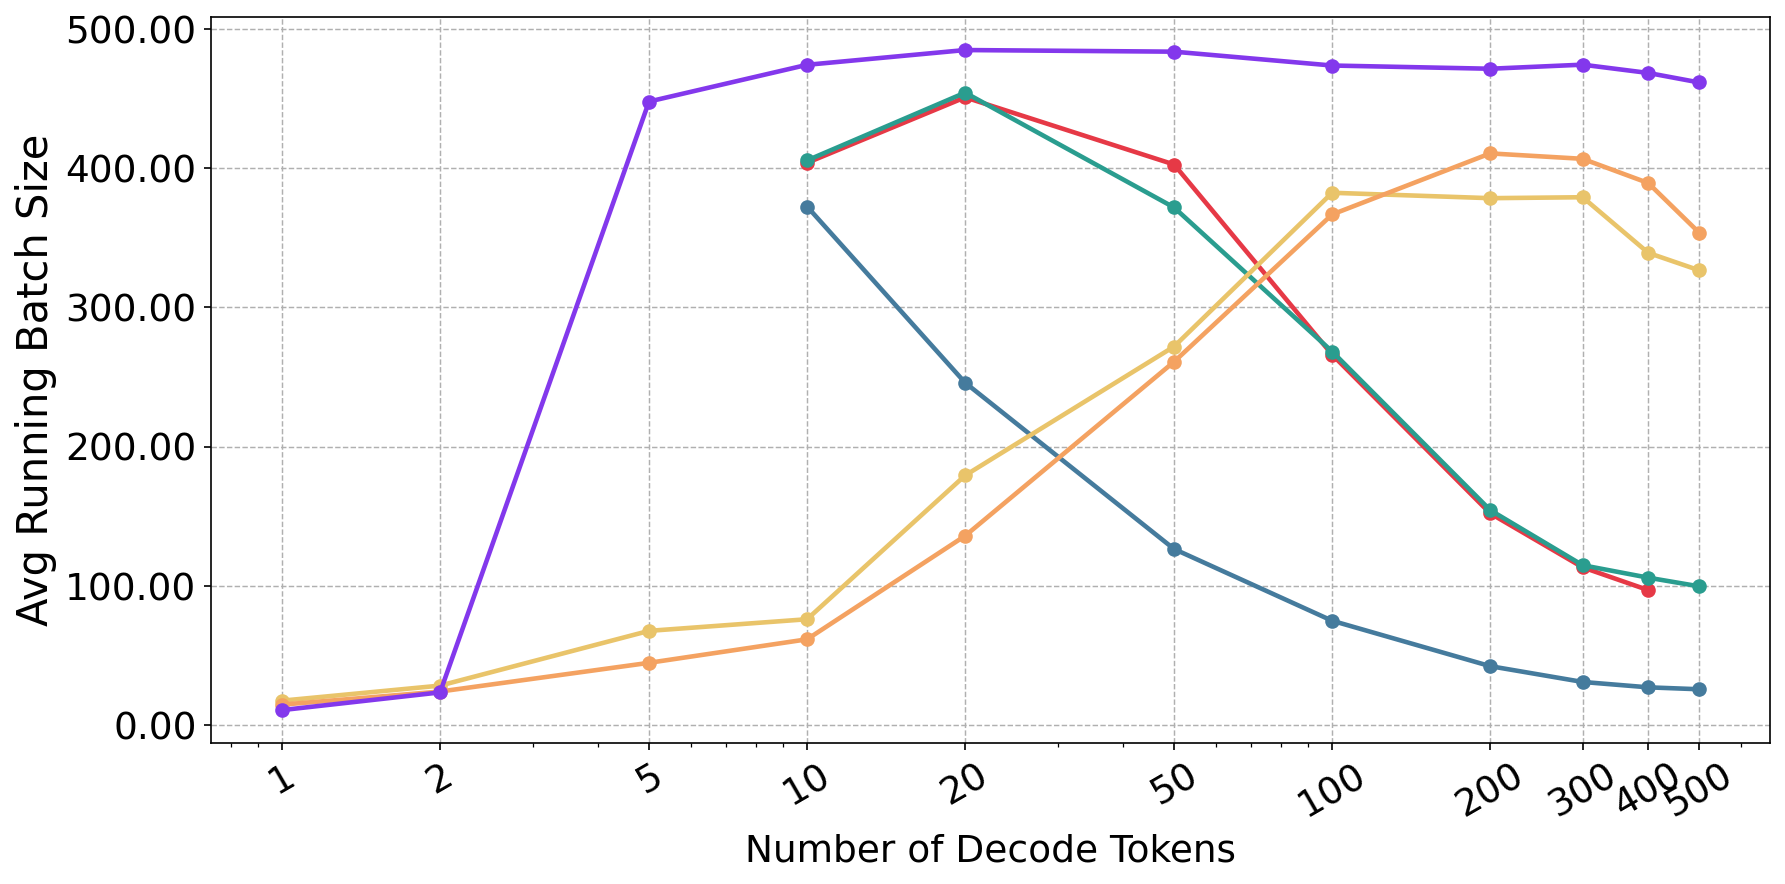
\includegraphics[width=\linewidth]{results/decode_tokens_plots/avg_batch_vs_tok.png}
    \caption{}
    \label{fig:tbt_vs_tok_l_5000}
\end{subfigure}
\hfill
\begin{subfigure}{0.32\textwidth}
    \centering
    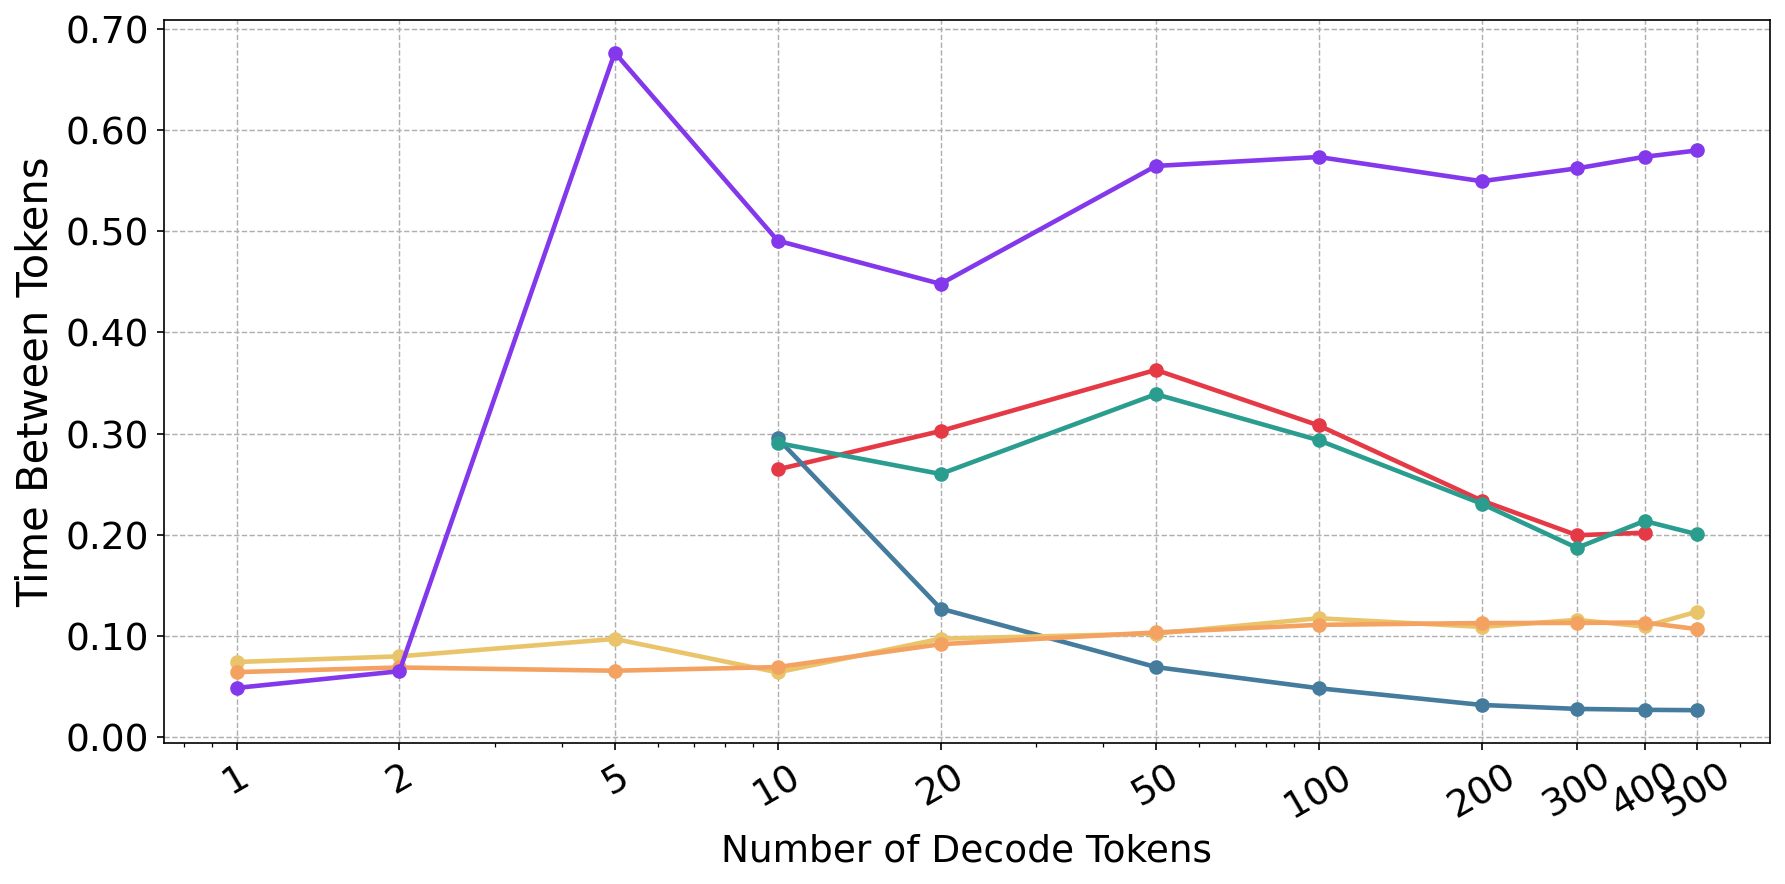
\includegraphics[width=\linewidth]{results/decode_tokens_plots/avg_timediff_vs_tok.png}
    \caption{}
    \label{fig:abs_vs_tok_l_5000}
\end{subfigure}

\caption{Various metrics across varying number of total decode tokens. Shared prefix length of 5000 tokens; 500 input request poisson rate and 5 prefix groups.}
\label{fig:metrics_vs_tok_l_5000}
\end{figure*}

\begin{figure*}[t]
\centering
\begin{subfigure}{0.32\textwidth}
    \centering
    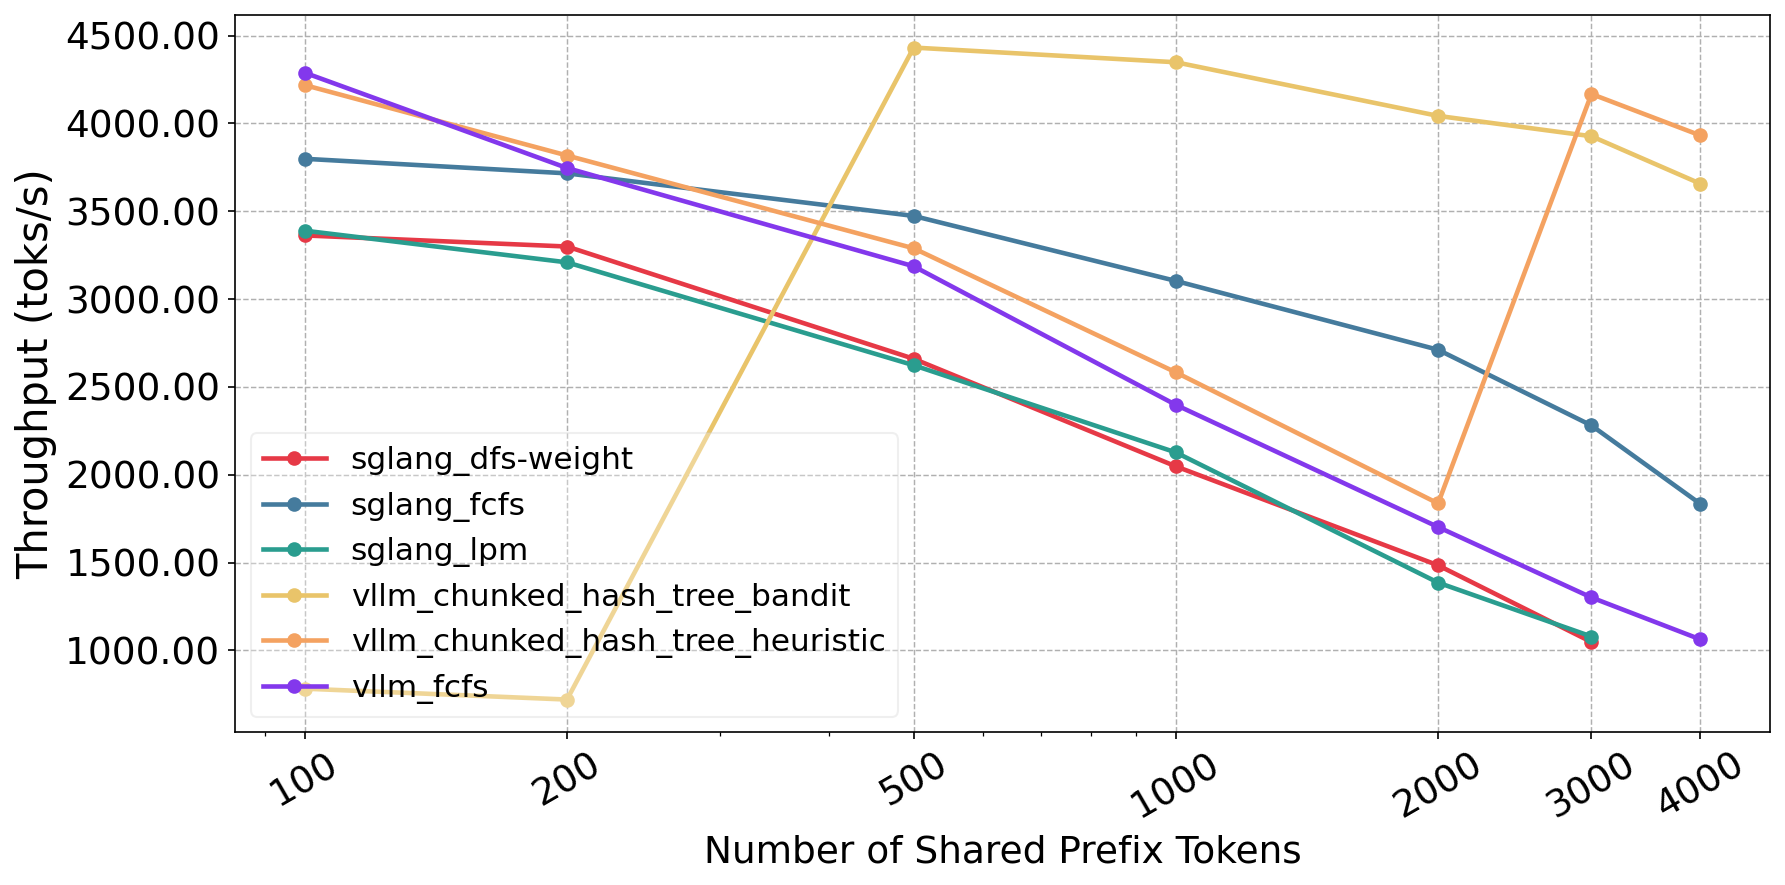
\includegraphics[width=\linewidth]{results/sys_prompt_tokens_plots/throughput_vs_sys_prompt_tokens.png}
    \caption{}
    \label{fig:tp_vs_sys}
\end{subfigure}
\hfill
\begin{subfigure}{0.32\textwidth}
    \centering
    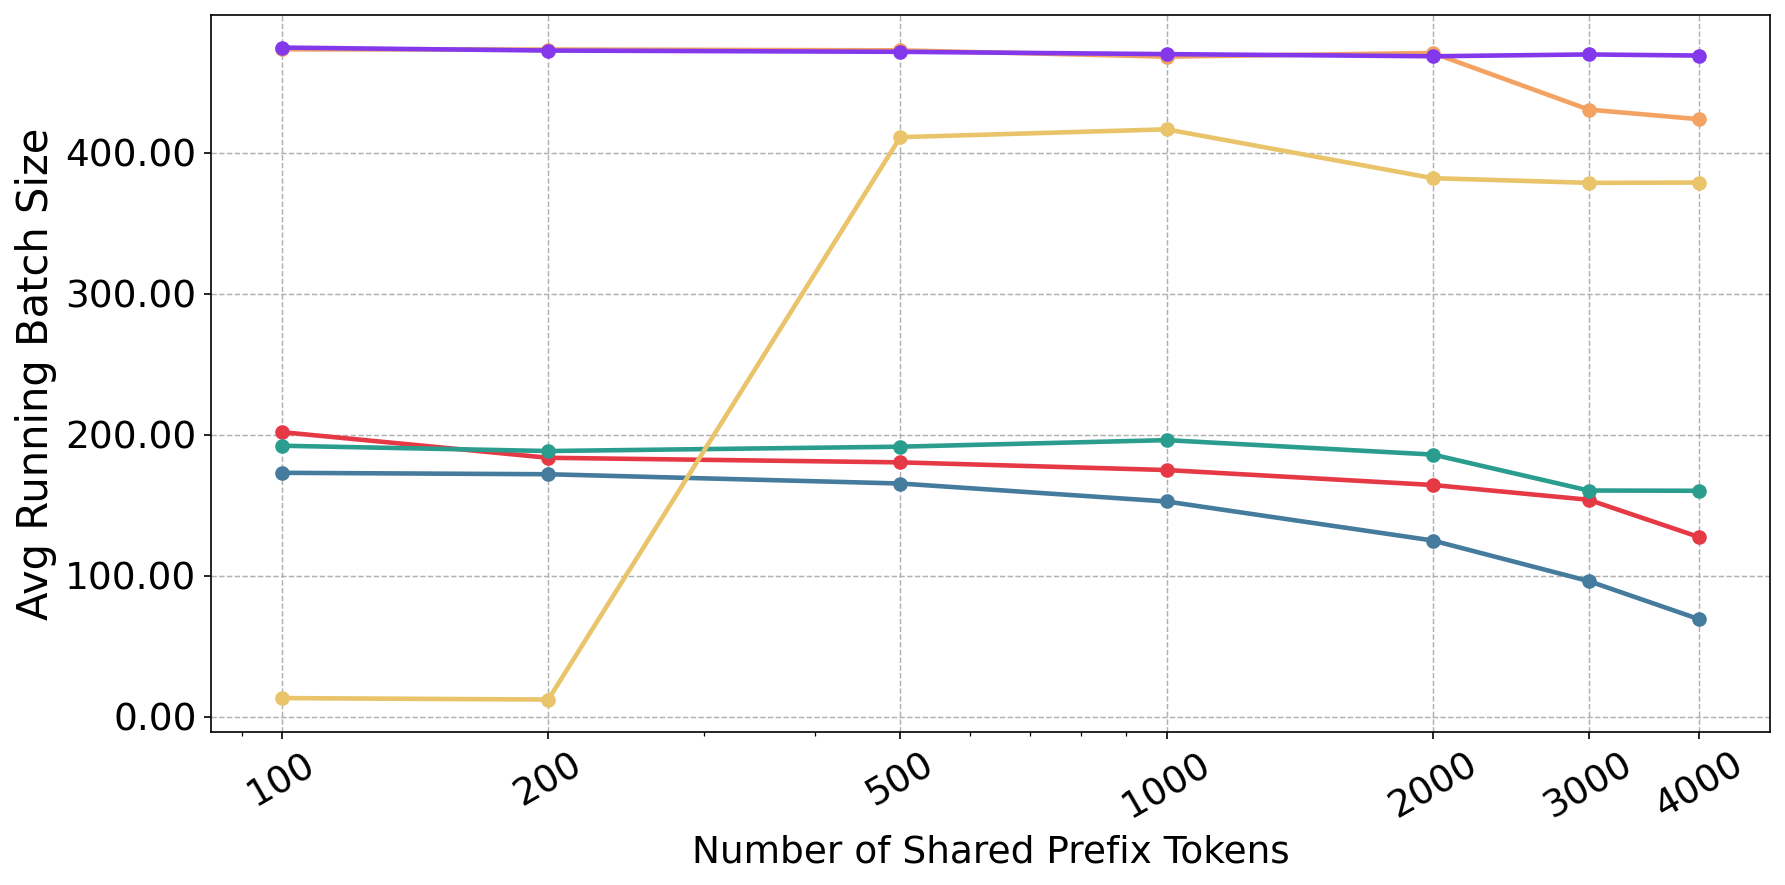
\includegraphics[width=\linewidth]{results/sys_prompt_tokens_plots/avg_batch_vs_sys_prompt_tokens.png}
    \caption{}
    \label{fig:tbt_vs_sys}
\end{subfigure}
\hfill
\begin{subfigure}{0.32\textwidth}
    \centering
    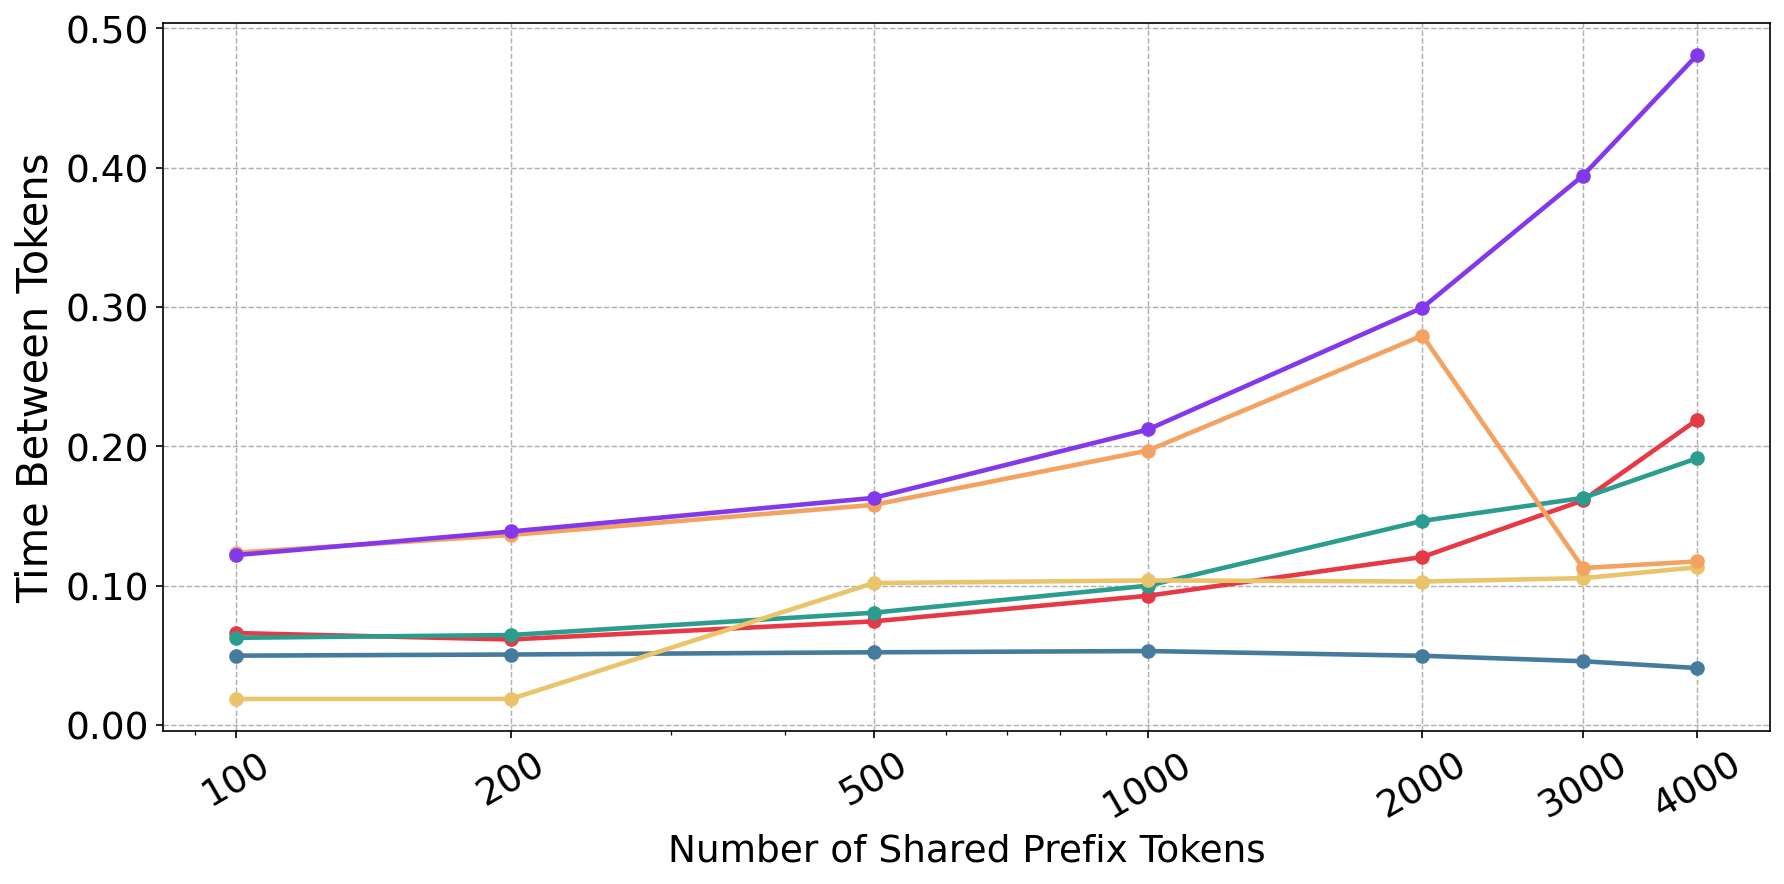
\includegraphics[width=\linewidth]{results/sys_prompt_tokens_plots/avg_timediff_vs_sys_prompt_tokens.png}
    \caption{}
    \label{fig:abs_vs_sys}
\end{subfigure}

\caption{Various metrics across varying number of shared prefix tokens. 200 tokens decode length; 500 input request poisson rate and 5 prefix groups.}
\label{fig:metrics_vs_sys}
\end{figure*}

\textcolor{red}{add many more results - on TBT, normalized latency, out tokens/sec?}

